% For formatting purposes only 
\setcounter{chapter}{8}
\setcounter{section}{3}
\setcounter{subsection}{0}
%\listofalgorithms - think about it ...
%--------------
%- COPY START -
%--------------
\paragraph{Decision Frame:} The \emph{mission control run} (fig. \ref{fig:missionControlRunActivityDiagram}) describes overall process in \emph{sequence}. The \emph{orchestration overview} is given in (fig. \ref{fig:misisonControlRunOrchestrationDiagram}).

The key idea is to explain what happen in one \emph{decision frame}. The \emph{mission control run} is implemented as multi-thread application which sends the signals between threads. Each thread is semi-independent process with forced synchronization on \emph{decision frame switch}.

\begin{figure}[H]
    \centering
    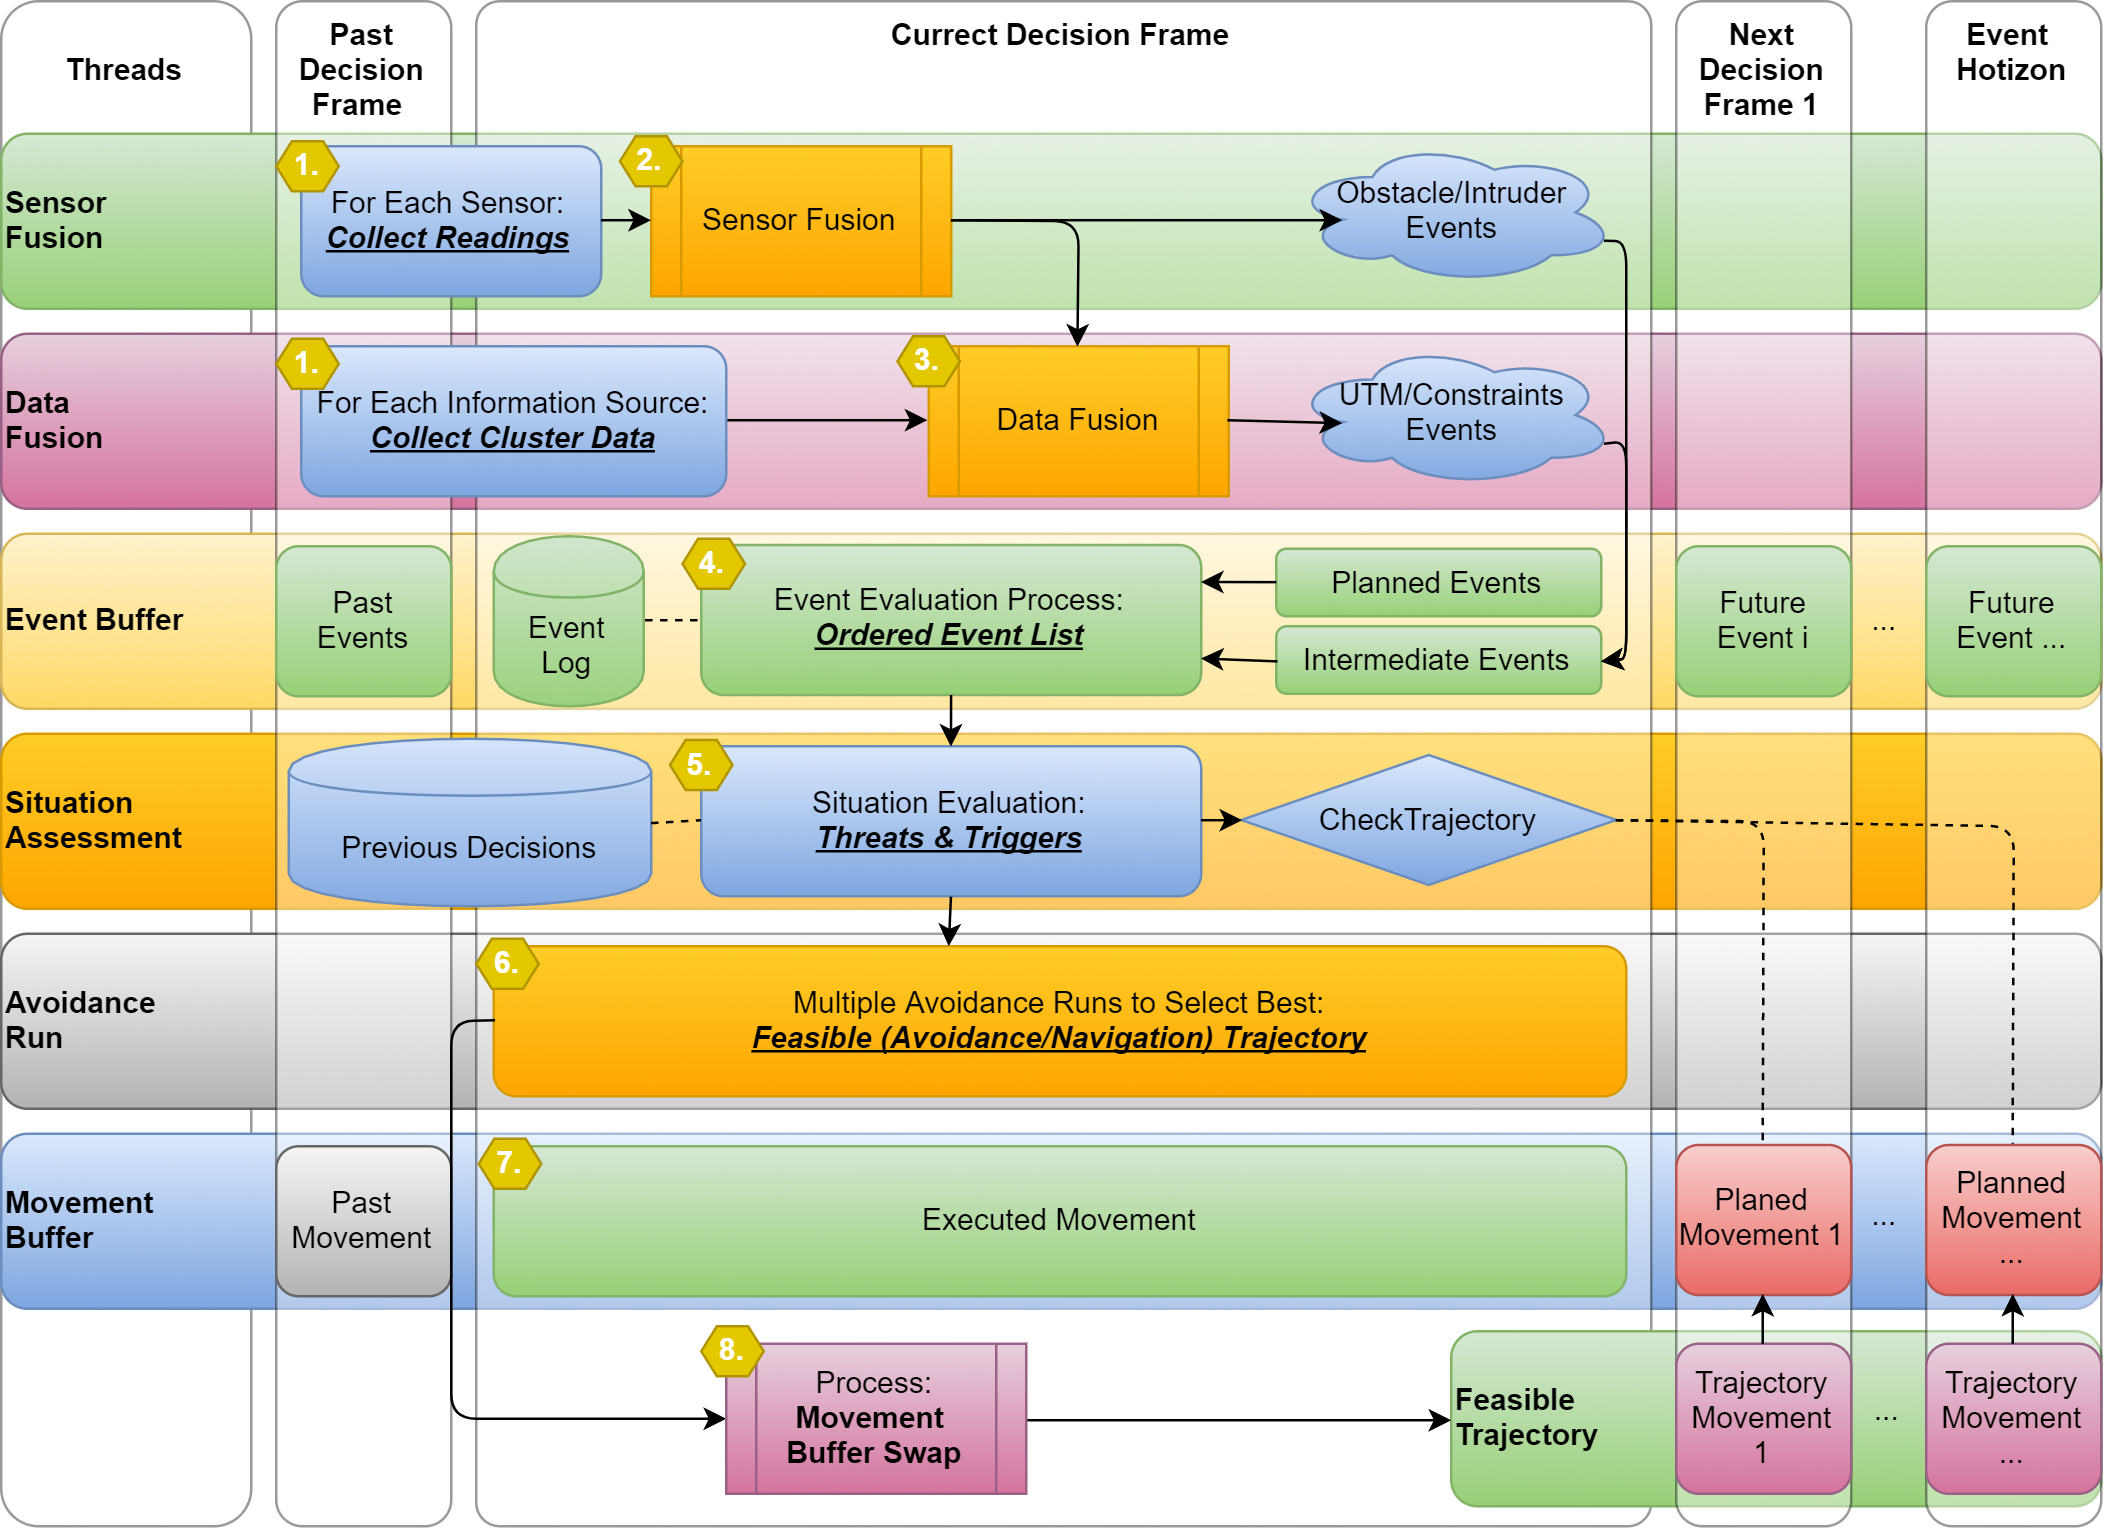
\includegraphics[width=\linewidth]{\FIGDIR/TE064DecisonFrameExplained}
    \caption{Mission control orchestration diagram.}
    \label{fig:misisonControlRunOrchestrationDiagram}
\end{figure}

\noindent The notable threads and their roles \& responsibilities are summarized like follow:
\begin{itemize}
    \item[1.] \emph{Sensor Fusion} - responsible for processing real time sensor array (sec. \ref{s:SensorFusionDefinition}). The output is partial known world assessment (sec. \ref{s:KnownWorld}). An \emph{obstacle detection} and \emph{intruder detection} events can be risen by this thread. 
    
    \item[2.] \emph{Data Fusion} - responsible for enhancing data from \emph{sensor fusion} by mixing data originating from \emph{information sources} (sec. \ref{s:dataFusionDefinition}). The information sources used in this work contains constraints originating from \emph{geo-fencing}, \emph{weather}, \emph{airspace restrictions}. This thread is delayed by \emph{sensor fusion}. A \emph{data fusion procedure} strongly depends on \emph{operational space context} (controlled/non-controlled airspace). The output of \emph{data fusion} is full \emph{known world assessment} (sec. \ref{s:KnownWorld}, \ref{s:sensorFusion}). The \emph{UTM-related} and \emph{constraint related} events can arise from \emph{data fusion}.
    
    \item[3.] \emph{Event Buffer} -  special data structure to store, raise, handle, prioritize events raised by other threads. 
    
    The \emph{implemented events} are listed in 5\textsuperscript{th}-6\textsuperscript{th} step of \emph{mission control run}. The events can be categorized like follow:
    \begin{itemize}
        \item[a.] \emph{Planned events} - raised in previous decision frames to be executed in actual or future \emph{decision frame}. 
        
        \item[b.] \emph{Intermediate events} - raised in \emph{actual decision frame} by other threads to be solved intermediate. 
    \end{itemize}
    
    The event buffer thread executes following event-related activities:
    \begin{itemize}
        \item[a.] \emph{Storing} - the \emph{events} are stored in \emph{event log}. The trace is useful for process and rule fine-tuning. 
        
        \item[b.] \emph{Raising} - the combination of events (multiple avoidance events) (example sec. \ref{s:testRuleMixed}) can trigger additional avoidance behaviour in form of combined-event.
        
        \item[c.] \emph{Handling} - the events are handled by invoking the \emph{situation assessment} or by rule engine invocation (sec. \ref{s:RuleEngineArchitecture}).
        
        \item[d.] \emph{Prioritizing} - the multiple events can be risen during one \emph{decision frame}. Some events can not be merged and needs to have proper prioritization before handling, like the \emph{obstacle detection} events before \emph{intruder detection event}.
    \end{itemize}
    
    \item[4.] \emph{Situation Assessment} - invoked by \emph{event buffer} o assess situation, responsible for proper \emph{avoidance run} (sec. \ref{s:aviudabceGridRun}) dataset preparation and invocation. The main responsibility is to check \emph{planned trajectory feasibility} stored in \emph{movement buffer} as \emph{planned movements}.
    
    \item[5.] \emph{Avoidance Run} - invoked by \emph{necessity to plan trajectory} originating from \emph{event buffer} or \emph{situation assessment} threads. The avoidance run produces one or multiple \emph{avoidance/navigation} feasible trajectories according to  7\textsuperscript{th}-11\textsuperscript{th} step of \emph{mission control run}.
    
    \item[6.] \emph{Movement Buffer} - represents \emph{movement automaton implementation} (sec. \ref{s:movementAutomatonDefinition}). The movement automaton consumes \emph{movement automaton buffer} each decision frame contains exactly one \emph{movement}. The movements can be viewed as:
    \begin{itemize}
        \item[a.] \emph{Past movements} - already executed movements in \emph{past decision frames}.
        
        \item[b.] \emph{Executed movement} - actually executed movement in current decision frame, this movement can not be changed.
        
        \item[c.] \emph{Future movements} - future planned movements to be executed after \emph{current decision frame} expires. These movements outlines planned trajectory (predictor mode sec. \ref{s:referenceTrajectoryGenerator}).
    \end{itemize}
    
    \item[7.] \emph{Feasible Trajectory} - consists of \emph{future planned movements} taking place directly after \emph{correct decision frame}. If its necessary, the planned trajectory in movement buffer is no longer feasible, the planned movements will throw away and replaced by \emph{trajectory movements}. 
\end{itemize}

\noindent The \emph{roles \& responsibilities} of each thread have been explained to outline their orchestration and roles in \emph{mission control run} (fig. \ref{fig:missionControlRunActivityDiagram}). The numbered steps in (fig. \ref{fig:misisonControlRunOrchestrationDiagram}) shows the threads orchestration in following manner:

\begin{itemize}
    \item[1.] \emph{Sensor \& Data fusion data set preparation/collection} - the sensor readings are collected trough multiple past and over current \emph{decision frame}. Each sensor reading is filtered and processed according to best practices. 
    
    The raw information from various data sources is loaded for relevant space clusters. The relevant space clusters are determined based on \emph{UAS expected position}. 
    
    \item[2.] \emph{Sensor fusion} - the readings from sensors are preprocessed according to (sec. \ref{s:staticObstacles}, \ref{s:intruders}).
    
    \item[3.] \emph{Data fusion} - the information sources are preprocessed according to (sec. \ref{s:staticObstacles}, \ref{s:intruders}).
    
    \item[4.] \emph{Event evaluation process} - the events are evaluated, if there is any triggering event (5\textsuperscript{th}-6\textsuperscript{th} mission control run steps) the situation evaluation process is called.
    
    \item[5.] \emph{Situation evaluation process} - the situation is evaluated according to 5\textsuperscript{th}-6\textsuperscript{th} mission control run steps.
    
    \item[6.] \emph{Feasible trajectory selection process} - from collected \emph{navigation/avoidance trajectories} (7\textsuperscript{th}-10\textsuperscript{th} mission control run steps). If there are more feasible trajectories (increasing threat) the one compliant with the most of the threats is selected.
    
    \item[7.] \emph{Movement execution} - the movement for \emph{current decision frame} is being executed.
    
    \item[8.] \emph{Movement buffer swap} - if there is a new \emph{feasible trajectory} the future movements for next decision frames are flushed away. The movement buffer is then filled with \emph{feasible trajectory movements}.
    \begin{note}
        This step impacts the duration of future \emph{decision frames}.
    \end{note}
\end{itemize}